\clearpage
\chapter{Algorithm Design} \label{chap:algorithm}

The first step in applying a genetic algorithm to a problem is to define the
data structure that represents the solution to the problem. This study looks at
optimizing a game player that can play a game of Monopoly. So this chapter
starts with a study of the game and existing strategies, and use information
that to guide the development of a genome that represents the game strategy of a
player.

Next, the fitness functions are developed. As seen in
Chapter~\ref{chap:background}, when applying machine learning techniques to
games, it is often necessary to apply a competitive fitness function. For this
study some pure competitive fitness functions were developed, but other
techniques for measuring fitness that are not directly competitive were also
developed.

Finally, the mechanics of the evolution strategy are developed. The parameters
of the evolution can have a big impact on the results of the evolution. As just
one example, it is well understood that if a population is not allowed to evolve
through enough generations, the solutions that develop are not optimal; however
letting a population evolve for too long wastes computing resources.

\section{Game Strategy} \label{5_strategy}

Prior to designing a chromosome for the game strategy, a state machine was
developed for a prototype player (See Figure \ref{figure-statemachine}). In many
cases, the transition from state to state is made automatically without input
from the player. For example, from the Inactive state, the player always has to
roll the dice and move to a new location on the board (with the exception of
being in jail where the player must roll, but doesn't necessarily move); this
event does not require any input from the player. However, analysis of the state
machine revealed four state transitions that do require a decision on the part
of the player.

\begin{figure}[htp]
\centerline{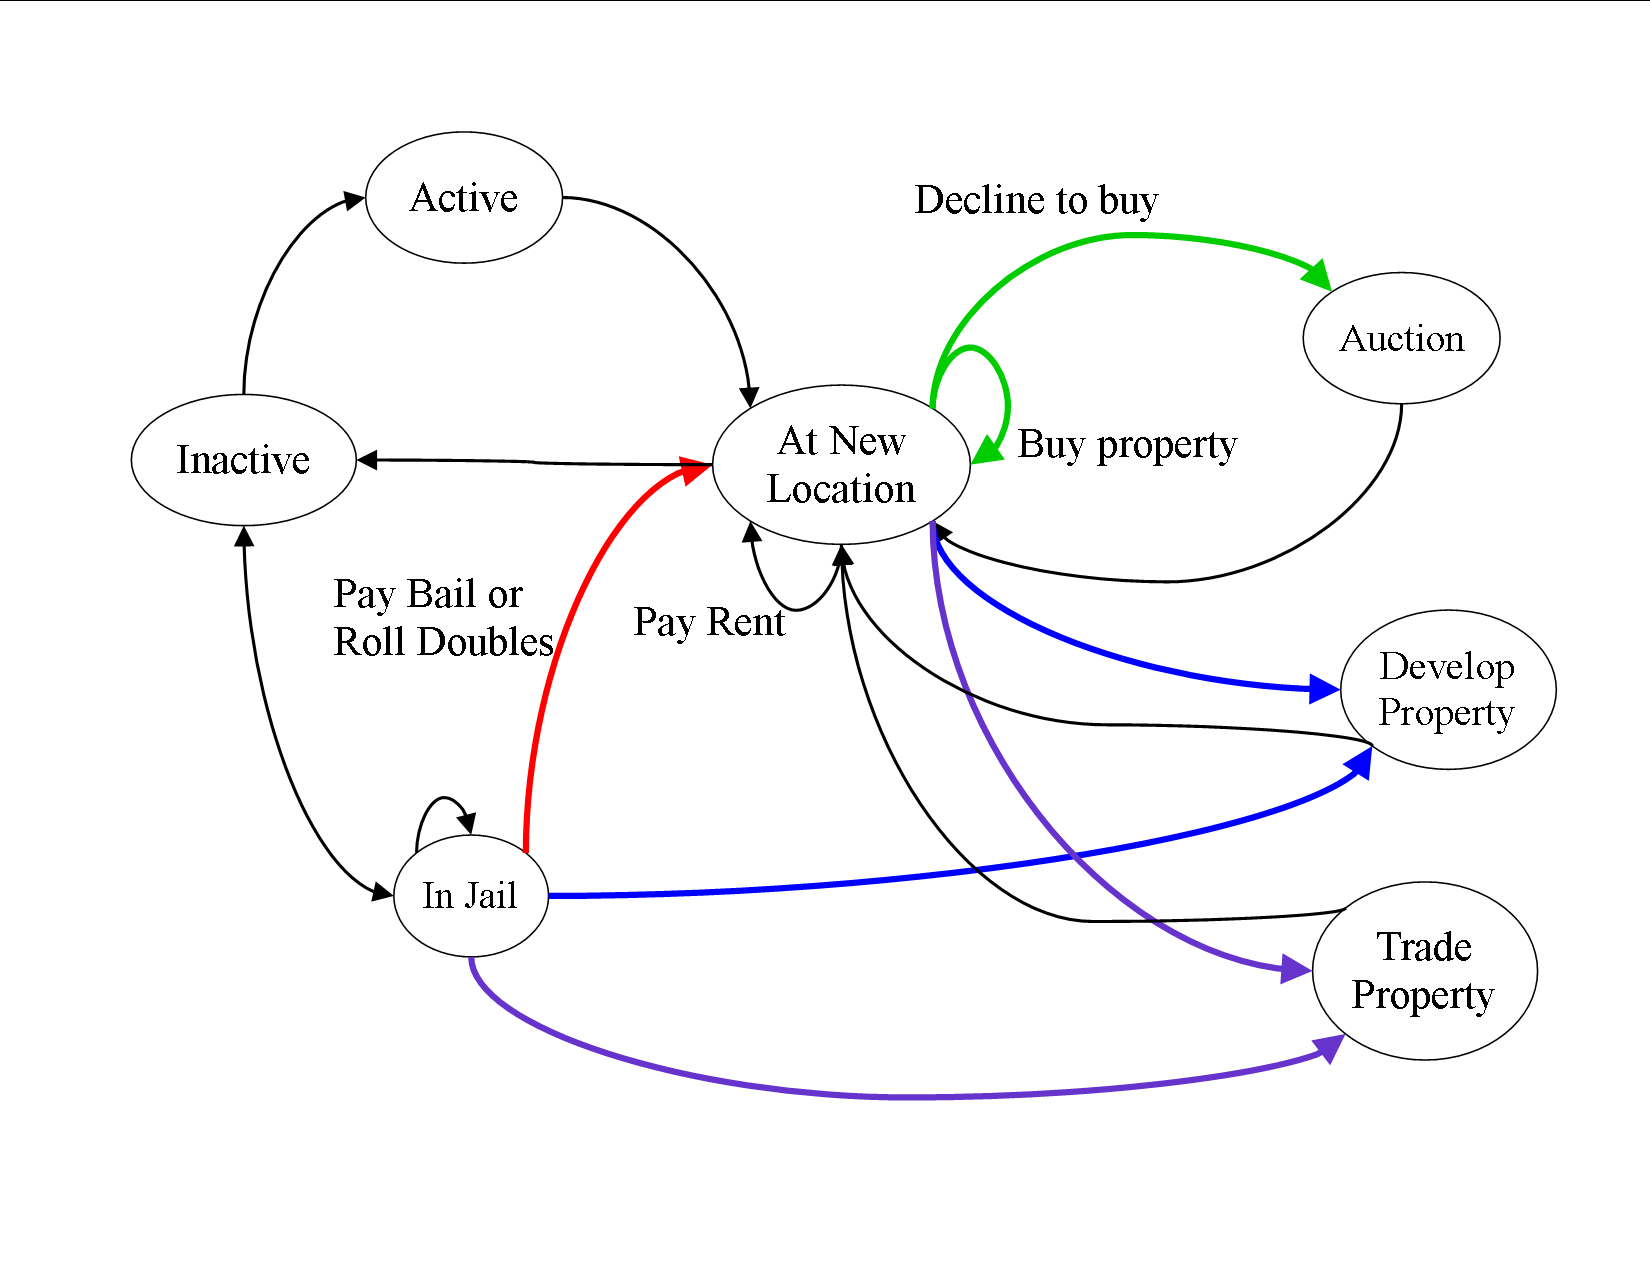
\includegraphics[width=1.0\columnwidth]{Figures/statemachine.png}}
\caption[Monopoly player state machine]{A simplified illustration of the state
machine for a prototype player. Not all state transitions are shown here; for
example, a player can participate in an auction from the inactive state.}
\label{figure-statemachine}
\end{figure}

The decisions that a player makes are whether to buy a property or not (the
arrows numbered 1 in Figure~\ref{figure-statemachine}), whether to pay bail to
exit jail or not (the arrows numbered 2 in Figure~\ref{figure-statemachine}),
whether to buy houses for a property or not (the arrows numbered 3 in
Figure~\ref{figure-statemachine}), and whether to trade a property or not (the
arrow numbered 4 in Figure~\ref{figure-statemachine}).

\subsection{Buying Property}
The primary objective of the game is to acquire and develop properties, and to
obtain monopolies of property groups. When a player lands on an unowned
location, the player must decide whether or not to buy the property. If the
player declines to buy the property, any player, including the player who
declined to buy the property originally, can bid for the property in an auction.
The player must then decide whether to participate in the auction and how much
to bid for the property.

Decisions on whether to buy a property depend on what other properties have been
acquired and which players have acquired them.
  
\subsection{Paying Bail}
When a player is in jail, the player must decide whether to pay bail and exit
jail immediately, or roll the dice and wait until doubles are rolled.

The decision of whether to stay in jail or leave jail depends on what other
properties have been acquired and which players have acquired them.

\subsection{Buying Houses or Hotels}
When a player has a monopoly, the player must decide when and how to buy houses
or hotels for their properties. There are a limited number of buildings in the
game. Whether a player can build depends on what other players have built, and
vice versa.

\subsection{Trading Properties}
The ability to develop a property group depends on the ability of the player to
acquire all the properties in a group. This is done by trading with other
players. When some other player owns one or more properties needed to complete a
monopoly, the player must decide if and when to trade for properties to complete
a monopoly.

\subsection{General Approach}

The four decision areas above led to a preliminary decision to use a multiple
chromosome strategy where different chromosomes will control the player behavior
depending on the state of the game: one strategy for early in the game when few
properties are owned; a different strategy for later in the game when many
properties are owned. Frayn used a similar strategy, except in his study
chromosomes represented the valuation of properties, which depended on ownership
and development factors~\cite{DBLP:conf/cig/Frayn05}. Also, Frayn used only
three chromosomes for house valuations.

Additionally, this study used genetic algorithms for just two decisions the
player would make: the buy property decision and the get out of jail decision.
The Get Out Of Jail chromosome is another departure from Frayn; from his paper,
it appears that Frayn's Get Out Of Jail decision was based on two genes from a
chromosome that also controlled other game decisions.
 
The other two decisions, whether to build a house and whether to trade a
property, were not implemented using genetic computation. The house buying
decision was implemented as a rule based algorithm and is discussed further in
section~\ref{5_buy_house}. The property trading decision was implemented by
adapting a property evaluation function proposed by Yasumura, Oguchi, and
Nitta~\cite{Yasumura2001Negotiate}. The property trading decision is discussed
in Section~\ref{5_trade_property}.

\section{Chromosome description} \label{5_chromo}

The genome for the evolved player consists of multiple chromosomes, each
chromosome used for a different purpose or state of the game. This is in
contrast to the classic simple GA (SGA) where each member of the population has
a single chromosome that is expressed as a string of binary
digits~\cite{haupt2004practical}. Following the initial description of the
genome used in this study, two alternate versions of the chromosome will be
described.

\subsection{Chromosomes for Buying Property}

After deciding on a multi-chromosome representation for an individual, the
structure of those chromosomes was designed. Considering that one set of
chromosomes would be used to control whether to buy a property, and that there
are four states a property group can be in, it was decided that the first set of
chromosomes would consist of 4 arrays of real numbers, 40 elements per array
(See Table \ref{table-chromo}). This chromosome is referred to as the RGA Player
(RGA for Real-valued Genetic Algorithm). Each element of the array represents
the probability that the player will purchase the property represented by the
array element. There are 40 locations on the Monopoly board, so each location
corresponds to an element in the array. The ``Go'' space is element 0, with
subsequent locations assigned successive element indices.
However, only 28 locations can be owned by a player, so 12 of the array elements
are ignored.\footnote{The chromosome could have been designed with only 28
locations, but by using 40 elements, the need to create a mapping between
locations and array elements is avoided (improved code readability and
maintainability) at a small cost of memory for the 12 unused elements.}

Each array corresponds to one of the following game states:

\begin{enumerate}
  \item{The first array is used when no player owns any property in the group
  where the player is currently located.}
  \item{The second array is used when the current player owns at least one
  property in the group where the player is currently located and no other
  player owns property in that group.}
  \item{The third array is used when one other player owns property in the
  property group where the player is currently located.}
  \item{The fourth array is used when two other players both own property in the
  property group where the player is currently located.}
\end{enumerate}

\begin{table}[ht]
\caption{Chromosome Illustration}
\begin{center}
\begin{tabular}{|l|c|c|c|c|c|}
\hline
\multicolumn{1}{|l|}{\backslashbox{Location}{Chromosome}}
& \multicolumn{1}{|c|}{Chr1}
& \multicolumn{1}{|c|}{Chr2}
& \multicolumn{1}{|c|}{Chr3}
& \multicolumn{1}{|c|}{Chr4} 
& \multicolumn{1}{|c|}{Etc\ldots } \\ \hline
0 - Go &  ignored  &  ignored &  ignored & ignored & \ldots \\ \hline 
1 - Mediterranean Ave &  $0.615$  &  $0.540$  &  $0.611$ & $0.654$ & \ldots \\ \hline 
2 - Community Chest &  ignored  &  ignored &  ignored & ignored & \ldots \\ \hline 
3 - Baltic Ave &  $0.288$  &  $0.532$  &  $0.165$ & $0.088$ & \ldots \\ \hline
4 - Income Tax &  ignored  &  ignored &  ignored & ignored & \ldots \\ \hline
5 - Reading Railroad & $0.129$  &  $0.649$  &  $0.965$ & $0.390$ & \ldots \\ \hline 
6 - Oriental Ave & $0.834$  &  $0.310$  &  $0.593$ & $0.738$ & \ldots \\ \hline
Etc\ldots & \ldots & \ldots & \ldots & \ldots & \ldots \\ \hline
\end{tabular}
\label{table-chromo}
\end{center}
\end{table}

Each gene in the chromosome represents the probability that the player will make
a positive decision. That is, when the player lands on an unowned street
location, the player must decide whether or not to buy the street. A random
number is generated, and if that random number is less than the gene value, the
player has ``decided'' to buy that street.

Based on the game strategies listed earlier (Section \ref{m_gamestrategies}),
the 4th chromosome will tend to have values that are generally less than the
values in the 1st, 2nd and 3rd chromosomes. That is, the player will tend to
decide to buy property more often when no other player owns any properties in
the group (1st chromosome), and when the property is needed to complete a
monopoly (2nd chromosome), and when the property is needed to block another
player (3rd chromosome).

\subsection{Chromosomes for Paying Bail}

The other set of chromosomes is used to determine when to pay to get out of
jail, and when to remain in jail (and hopefully not roll doubles with the dice).
This chromosome is a 2-D array of real numbers.

Rows and columns in the array are indexed by 6-bit numbers created by the
properties on one side of the board. The first index corresponds to the west
side of the board; the second index corresponds to the north side of the board.
These are the sides of the board on which the player is most likely to land
immediately after leaving jail. For each property on the west or north side of
the board, the corresponding bit in the index is set to 1 if the property is
owned by some other player; otherwise, it is set to 0. For example, there are
six properties on the west side of the board. In board order they are St Charles
Place, Virginia Ave, States Ave, St James Place, New York Ave, and Tennessee
Ave. If opponents owned the first three, the index would be $000111_2$. The
second index is formed similarly. The two indices are then used to access an
element in the array.

The value at the element is a real number which represents the probability that
the player will choose to pay the bail. When the player is in jail, if a
randomly generated number is less than the gene value, the player has ``decided"
to pay bail. Note that this scheme automatically accounts for different game
states:
early in the game very few of the properties are owned (none when the game
begins) so the indices will be near (0, 0); later in the game, if many
properties are owned by other players, the indices will be near (63, 63). It
also accounts for differences in ownership. That is, if opponents own many
properties on the West and North edges, the indices will be relatively high,
whereas if the player owns many of the properties, the indices will be
relatively low. So, if the player owns properties near the jail, his jail
decision will be similar to the decision made early in the game when few
properties are owned.

\subsection{Alternate Chromosome for Paying Bail} \label{5_altjail}

Because the 64x64 array described above consumes a relatively large amount of
memory, this study also looked at an alternate genome which varied this
chromosome by making it a 4x4 array. Instead of indexing by which players owned
properties on the west and north edges of the board, the indices were created by
determining if any of the four color groups on the west and north edges are part
of a monopoly owned by an opponent. This only requires a two-bit index and 16
array elements. The players that use this alternate Jail chromosome will be
referred to as the TGA Players\footnote{Unlike the R (for Real) in RGA, or the S
(for Simple) in SGA, the T in TGA has no meaning. It was chosen because it
follows R and S alphabetically.}.

\subsection{Alternate Chromosome description} \label{5_altchromo}

Goldberg described the chromosome structure of the SGA in \emph{Genetic
Algorithms in Search, Optimization, and Machine
Learning}~\cite{goldberg1989genetic}. The SGA uses a single string of binary
bits for its chromosome. Although the primary population used in this thesis
consists of real valued chromosomes described above, the same information could
be encoded into a binary strings.

Start by representing a decision as a 6-bit gene. If each gene is interpreted as
an integer, then each gene will have some value from 0 to 63. Each value is also
interpreted as the chance of making a positive decision. Just as with the RGA
chromosome, when a decision is required, a random integer between 0 and 63
inclusive is generated; if that random value is less than the chromosome value,
the player has ``decided'' to buy the property. Thus, each gene has a coarseness
of approximately 1.56\% for each decision.

All the genes are concatenated into a single string. So, for example, the first
chromosome of 40 elements in the RGA becomes a single string of 240 bits (6 bits
* 40 elements). Each of the other property buying chromosomes is encoded in the
same way.

Likewise, the 4x4 chromosome for paying bail is then encoded as a 96 bit string
(16 genes x 6 bits per gene). This chromosome uses the simplified indexing
scheme described previously in section~\ref{5_altjail}.

A population of these individuals, referred to as Simple GA (SGA) Players, was
also simulated in this study.

\section{House buying algorithm} \label{5_buy_house}

The decision of when to buy houses or hotels was implemented using a simple rule
based procedure. The procedure is summarized in Algorithm~\ref{alg_buyHouse}.

\begin{algorithm}
\caption{House Buying Algorithm}
\label{alg_buyHouse}
\begin{algorithmic}
\IF{not player has monopoly} 
  \STATE exit
\ENDIF

\IF{not player has sufficient cash} 
  \STATE exit
\ENDIF

\WHILE{player has sufficient cash}
  \IF{player has less than 3 houses on all monopolies}
    \STATE buy house for a property with less than 3 houses
  \ELSE
    \STATE buy 4th house or a hotel for a property
  \ENDIF
\ENDWHILE
\end{algorithmic}
\end{algorithm}

The algorithm begins by checking that the player has a monopoly. If the player
does not have a monopoly, the algorithm exits since the player cannot buy
houses.

Then the algorithm checks that the player has enough cash. A variation 
of Frayn's procedure for computing the minimum cash a player should keep
available was used~\cite{DBLP:conf/cig/Frayn05}. A player should keep
\$200 plus 1\% of the total net worth of all players in the game
plus 1\% of the average net worth of the players in the game plus 10\% of the
cost of all houses and hotels currently on the board.
\begin{equation*}
200 + 0.01 \cdot totalNetWorth + 0.01 \cdot avgNetWorth + 0.1 \cdot costOfHouses
\end{equation*}
For the player to have enough cash to buy a house or a hotel, the player must
have the minimum cash plus enough to buy a house or hotel for whichever
monopolies the player owns. If the player does not have enough cash, the
algorithm exits.

If the player has enough cash, the player buys houses for all monopolies
that have less than 3 houses on them\footnote{The greatest return for a player
occurs when building 3 houses on all properties, and not building 4 houses or a
hotel until all monopolies have 3 houses~\cite{orbanes2007monopoly}.}. If the
player has more than one monopoly, houses are bought for groups in this order:
Orange, Light Blue, Red, Purple, Dark Blue, Yellow, Green, Brown. This order was
chosen based on previous statistical analysis of the value of various property
groups~\cite{Ash1972,Abbott1997,DBLP:conf/cig/Frayn05}. If all monopolies owned
by a player have at least 3 houses on all properties, the algorithm will buy a
4th house, and then a hotel for the properties owned by the player.

\section{Property Trading Algorithm} \label{5_trade_property}

For the evolutionary phase of this research, the genetic algorithm players
played without the ability to trade properties. This allowed the players to
evolve strategies for buying properties independent of the option for trading
properties. With the ability to trade, players might have learned to decline
better properties in the expectation that the property could be acquired later
through a trade. Also, players might learn to buy less valuable properties at a
higher rate than expected so that the properties could be traded.

However, when it came time to play-test the GA players against human players, a
trading algorithm was needed so that human players would not be bored by a game
that was simply about which player was luckiest in landing on valuable
properties, or which player was lucky enough to acquire a monopoly by chance.

A trading algorithm based on research by Yasumura, et
al,~\cite{Yasumura2001Negotiate} was used as the basis for property trading by
the A.I. players in the human-A.I. competition. The human players were, of
course, free to use their own criteria for evaluating whether or not to trade
properties. Yasumura, et al,
developed an evaluation function that was the sum of some combination of
expected gains (Algorithms~\ref{alg_stg}, \ref{alg_mtg}, and \ref{alg_ltg})
minus expected losses (Algorithms~\ref{alg_stl} and \ref{alg_mtl}). The
ownership situation of the properties (See Algorithm~\ref{alg_bigU}) determines
how the gains and losses are summed. The player's decision is be based on the
result of the evaluation function and whether the player was weighted more
towards avoiding losses or seeking gains.

Expected short term gain \(E_S\) for player \(s\) getting a property card in a
trade is the sum of the probabilities that another player \(i\) will land on the
traded property or one of the properties in the same group in one dice throw
(\(P_S(i)\)) multiplied by the rental fee of the color group (\(R(M)\)) if the
owner used all their available cash \(M\) to buy houses for the color group.
\begin{algorithm} 
\caption{Compute Short Term Gain}
\label{alg_stg}
\begin{algorithmic}
   \STATE $E_S \gets \sum P_S(i) \cdot R(M)$ 
\end{algorithmic}
\end{algorithm}

Expected mid term gain \(E_M\) is the sum of the probabilities that another
player will land on the traded property or one of the properties in the same group in
one trip around the board multiplied by the rental fee of the color group if the
owner were used all their available cash to buy houses for the color group.
\begin{algorithm} 
\caption{Compute Mid Term Gain}
\label{alg_mtg}
\begin{algorithmic}
   \STATE $E_M \gets \sum P_M(i) \cdot R(M)$ 
\end{algorithmic}
\end{algorithm}

Expected long term gain \(E_L\) is the sum of the probabilities that another
player will land on the traded property or one of the properties in the same
group in one trip around the board multiplied by the rental fee of the color
group if the owner had \$1000\footnote{This is the value used by Yasumura, et
al. Their paper does not explain why this amount was chosen for computing long
term gain.} to buy houses for the color group.
\begin{algorithm} 
\caption{Compute Long Term Gain}
\label{alg_ltg}
\begin{algorithmic}
   \STATE $E_L \gets \sum P_M(i) \cdot R(1000)$ 
\end{algorithmic}
\end{algorithm}

The short term loss is simply the probability that the player \(s\) making the
trade will land on the property being traded on the next dice roll, multiplied by the
rent for that property if the new owner used all their cash to buy houses for
that property.
\begin{algorithm} 
\caption{Compute Short Term Loss}
\label{alg_stl}
\begin{algorithmic}
   \STATE $L_S \gets P_S(s) \cdot R(M)$ 
\end{algorithmic}
\end{algorithm}

The potential mid-term loss is the probability that the player \(s\) making the
trade will land on the location in one trip around the board multiplied by the rent
for that property.
\begin{algorithm} 
\caption{Compute Mid Term Loss}
\label{alg_mtl}
\begin{algorithmic}
   \STATE $L_M \gets P_M(s) \cdot R(M)$ 
\end{algorithmic}
\end{algorithm}

Finally, the various expected gains and losses are summed based on the property
ownership situation. There are 4 cases to evaluate: 1) the player \(s\) would
receive one card \(c\) of a given color group; 2) the player would have all
cards but one in a color group and the last card is in the bank; 3) the player
would have cards from a group, and another player would have the remaining
card(s); or 4) the player would have a monopoly after the trade.
\begin{algorithm} 
\caption{Evaluate Property}
\label{alg_bigU}
\begin{algorithmic}
  \IF {Case~1}
    \STATE $f(c) \gets \phi(c) \gets 1/2 \cdot FV(c) + E_L(c)$ \\
    \COMMENT {FV(c) is the face value, or cost, of the property card \(c\)}
  \ENDIF
  \IF {Case~2}
    \STATE $f(c) \gets 2 \cdot \phi(c) + E_M(c)$
  \ENDIF
  \IF {Case~3}
    \STATE $f(c) \gets 2 \cdot \phi(c) + E_M(c) + E_S(c)$
  \ENDIF
  \IF {Case~4}
    \STATE $f(c) \gets 3 \cdot \phi(c) + E_M(c) + E_S(c)$
  \ENDIF
\\
  \REQUIRE $\omega_1 + \omega_2 = 1$
\\
  $U \gets \omega_1(\sum f(c) + M) - \omega_2(L_S + L_M)$
\end{algorithmic}
\end{algorithm}

After summing the gains, and weighting the sum by \(\omega_1\), the function
subtracts a weighted sum of the short-term and mid-term losses. The factor
\(\omega_1\) biases the function towards gain seeking; a high \(\omega_1\) means
the player will favor gains over avoiding losses. The factor \(\omega_2\) biases
the function towards avoiding losses; when \(\omega_2\) is high the player will
avoid trades that lead to potential losses. If the value of the function, \(U\)
exceeds a given threshold, the player will propose the trade, or accept a
proposed trade. 

Yasumura, et al, evaluated 5 thresholds from a low value of 100 to a high value
of 500. They developed a Monopoly simulator and competed various agents using
the simulator. They found the best profits and most wins were generated by
agents that used the lowest threshold. They also evaluated various values for
\(\omega_1\) and found the best results when \(\omega_1\) was greater the 0.5.
Following their lead, various values for the threshold and \(\omega_1\) were used 
for the human versus computer competitions. The results of these competitions
are discussed in detail in Sections~\ref{6_humanVRGA1} and \ref{6_humanVRGA2}.

\section{Fitness Evaluation} \label{5_fitnesseval}

Six different fitness evaluations were tested in the evolutionary process. Each
evaluator was applied separately to different populations. In 
Section~\ref{6_interpopValidation} the various evaluators are tested against 
each other and the results show which evaluators performed best.

Four of the fitness evaluations are based on which player wins a game, or in
which order the other players finish. The winner of a game is defined as the
last player left in the game, or the player with the greatest net worth when the
game finishes. The second place player is the second to last player in the game,
or the player with the second greatest net worth when the game finishes. Third
and fourth place players are determined similarly. The different evaluators
award fitness points to the players as follows.

\begin{enumerate}
  \item {Finish Order (FINISH\_ORDER); in a game with \(n\) players, the winner
  of the game receives \(n-1\) points; second place receives \(n-2\) points, and
  so on. The last place finisher receives 0 points.}
  \item {Number of Monopolies (NUM\_MONOPOLIES); each player receives one
  point for each monopoly they control.}
  \item {Number of Properties owned (NUM\_PROPERTIES); each player receives one
  point per property owned at the end of the game.}
  \item {Net Worth (NET\_WORTH); at the end of each game, the net worth of each
  player is calculated. Each player receives points that equal their net
  worth.}
  \item {Number of wins (NUM\_WINS); the winner of each game receives three
  points; all other players receive zero points.}
  \item {Tournament level (TOURNAMENT); players compete in a modified single
  elimination tournament. The fitness score is the level attained in the
  tournament tree.}
\end{enumerate}

Each player in a population competes in multiple games in every generation. Four
different values for number of games were used in the evolution process: 7, 25,
50, and 100 (See Section~\ref{5_compfit}). The player's total fitness for the
generation is the sum of the player's fitness score for each game after all
games in a generation are complete.

The fitness evaluators FINISH\_ORDER and NUM\_WINS were developed directly from
the work of Frayn, and indirectly from previous studies of genetic algorithms
and games. Frayn competed chromosomes against each other in four-player games.
The winner of each game received +3 points, the second place finisher received
+2, etc. This is very similar to the competitions discussed in
Chapter~\ref{chap:background}, where the winner in two-player games such as
Tic-Tac-Toe, Checkers, and Othello received points for winning a game, and the
loser received 0 points. Since Frayn used four players in each game, second and
third place finishers also receive some points (although less than the winner);
the last place finisher still gets 0 points. The FINISH\_ORDER fitness evaluator
uses the same 3/2/1/0 point scale to award scores in a game. NUM\_WINS  is a
simplified 3/0/0/0 fitness measurement where the winner receives +3 and every 
other player receives 0.

Players who win at Monopoly tend to acquire more
properties and more monopolies of properties. So two more fitness functions were
developed. One labeled NUM\_PROPERTIES that counts the number of properties that
a player owns and awards +1 point for each property. The other fitness function
is labeled NUM\_MONOPOLIES and it awards +1 points for each monopoly controlled
by a player.

Then there is a fitness function named NET\_WORTH. For each game played in the
simulation, the winner is the last one left in the game or the player with the
highest net worth (cash plus value of properties) in the game if not all players
go bankrupt. Thus the winner of the game will always have the highest net worth.
For each player in a game, NET\_WORTH computes the ratio of each player's net
worth to the total net worth of a game (the sum of the net worth of all the
players in the game). The ratio is then multiplied by 300 and the value is
awarded to the player as their score for the game.
\begin{equation*}
score = 300 \cdot net\_worth / total\_net\_worth
\end{equation*}
Last is the TOURNAMENT fitness evaluator (discussed in more detail
in~\ref{5_compfit}). A modified single elimination tournament is conducted in
each generation. The fitness score of each player is the level the player
attains in the tournament tree, starting at level 0. So, the losers of the first
round get a score of 0, and the winners get +1. This continues until only two
players remain.

The NUM\_WINS, FINISH\_ORDER, NET\_WORTH, and TOURNAMENT evaluators are the
evaluators that are direct competitive fitness functions. When using those
evaluators, the fitness of the players is based directly upon their performance
against other players.

The other two evaluators are only indirectly competitive. When players compete
against each other in the game, the winner of the game will probably 
acquire more properties or will acquire more monopolies than the other players.
So on average, the winning player of a game will have more properties or more
monopolies than the losing players. However, that is not necessarily the case.
as mentioned above, the winner of a game can be the player with the greatest net
worth. With NUM\_PROPERTIES and NUM\_MONOPOLIES, that the player with the
greatest net worth may not have the most properties or the most monopolies.

\section{Evolution and Propagation} \label{5_evoprop}

The parameters used in the genetic algorithm are based on the parameters used by
Frayn, with some modifications based on other research into coevolution,
competitive fitness functions, and games. Frayn's parameters for population evolution
are presented first, and then an explanation of the parameters
used in this project follows.

\subsection{Frayn's evolutionary parameters}

Table~\ref{table-fraynparams} shows the parameters that Frayn used when creating
and evolving the population of game players in his
research~\cite{DBLP:conf/cig/Frayn05}. His research used a competition method
similar to K-Random Opponents with \(K=300\), and a population size of 1000. As
mentioned previously, he used a single fitness measurement that awards points
based on the place-finish of each player in the game.

\begin{table}[ht]
\caption{Frayn's Evolution Parameters}
\begin{center}
\begin{tabular}{ | l | l | }
  \hline                        
  Population size: & 1000 \\ \hline
  Matches per generation: & 100 \\ \hline
  Number of players per game: & 4 \\ \hline
  Games per match: & 250 (1000 players/4 players per game) \\ \hline
  Fitness: & Game winner	+3 \\
  & Game 2nd place	+2 \\
  & Game 3rd place	+1 \\
  & Game 4th place	+0 \\
  & (Max score per generation is 300) \\ \hline
  Reproduction: & Elitism and reproduction, with crossover and mutation \\ \hline  
\end{tabular}
\label{table-fraynparams}
\end{center}
\end{table}

Frayn's process was as follows. 

\begin{enumerate}
  \item Initialize a population of 1000 individuals.
  \item Each individual plays 100 games.
  
  \begin {itemize}
    \item The 1000  individuals are randomly divided into 250 sets of 4.
    \item These 250 sets each play a game. Points are awarded at the end of the
    game.
    \item After all 250 games are complete, the 1000 individuals are again
    randomly divided into 250 different sets, and the sets play again.
    \item Repeat until each individual has played 100 games.
  \end{itemize}
  
  \item At the end of the generation, the total number of points earned by each
  individual is evaluated as the fitness of the individual.
  \item The new population of 1000 players is created.
  \begin{itemize}
    \item Top 3 players move into next generation (elitism).
    \item 300 players chosen by tournament selection with replacement.
    \item 300 players chosen by tournament selection with replacement and then
    mutated.
    \item 397 children created by selecting parents using tournament selection
    with replacement, and then applying uniform crossover to the parents'
    chromosomes.
  \end {itemize}
\end{enumerate}

Note that each player in a generation plays 100 games against 300 other
opponents (3 different opponents for each game). So the competitive fitness
function used by Frayn is K-Random Opponents with \(K\approx300\). K is
approximate because the three opponents are selected independently for each
game, so it is possible for the same opponent to be selected in more than one
game. Over the total span of his study, Frayn reported that his project included
over 377 million simulated games.

\subsection{Evolutionary parameters used in this research}

The last remaining task is to decide on the parameters to be used for the
genetic algorithm. The success of any genetic algorithm is highly dependent on
the parameters chosen. Parameters will be chosen using guidance from previous
studies. The thought is that if those parameters worked for previous studies
they will likewise lead to successful solutions in this study.

\subsubsection{Population size}

Chapter~\ref{chap:background} summarized several research studies that used
genetic algorithms to develop game players. When Fogel evolved neural networks
to play Tic-Tac-Toe, his population consisted of 50
individuals~\cite{Fogel1993}. The population for Checkers was 30
individuals~\cite{Fogel2000Anaconda,journals/tec/ChellapillaF01}.
The population for Othello was 20 individuals~\cite{ChongTW05}. When
Ja\'{s}kowski et al., introduced Fitnessless Coevolution, they used population
sizes comparable to those used in previous research that used the same
optimization problems~\cite{Jaskowski:2008:FC:1389095.1389161}.

This research uses a population size similar to Frayn's size of 1000. However,
to implement a modified single elimination tournament competition it will be
necessary to modify this value slightly to be 1024. Based on the results of the
studies of competitive fitness functions~\cite{Angeline:1993:CEE:645513.657590,
Panait02acomparative, Jaskowski:2008:FC:1389095.1389161}, the behavior of
smaller population sizes such as 32, 128, and 512 is also investigated.
The value 32 is chosen because it is similar to the population sizes of those
other studies; the other two sizes of 128 and 512 were chosen to provide
intermediate population sizes between 32 and 1024.

The initial assumption that valid results might be obtained with a population
size as small as 32 seems reasonable.
 Chapter~\ref{chap:background}
listed the state space complexity of various games to which genetic algorithms
had been applied. If the state space complexity of Monopoly is comparable to
those games, then the use of a small population size is a reasonable initial
assumption.

Note that there are 28 locations on the Monopoly board that can be owned by a
player. Any location can be unowned, or can be owned by one of the four players.
This gives an initial state space estimate of \(5^{28}\), or approximately
\(10^{19.6}\). This is within two orders of magnitude of Checkers at
\(\approx10^{18}\).

Now consider that houses can be built by a player on a property. Since houses
can only be built when one player owns all street locations in a property group,
only some state space configurations will allow houses or hotels. Assume
\(Player_{i}\) has a monopoly in the first or last color group on the board
(where there are two locations that can be built upon) and there are no other
monopolies. Then the number of additional state space configurations for either
group is
\begin{equation*}
4 \cdot 10 \cdot 5^{26} \approx 10^{19.8}
\end{equation*}
where 4 is the number of players that could have the monopoly, 10 is the number
of houses (2 streets with up to 4 houses or 1 hotel each), and \(5^{26}\) is the
state space for the remaining 26 locations on the board. If there is a single monopoly
in one of the other color groups (with 3 streets in the group), the
calculation is
\begin{equation*}
4 \cdot 15 \cdot 5^{25} \approx 10^{19.3}
\end{equation*}
So, considering just properties and single monopolies, the total state space
is
\begin{equation*}
5^{28} + (2 \cdot 4 \cdot 10 \cdot 5^{26}) + (6 \cdot 4 \cdot 15 \cdot 5^{25})
\approx 10^{20.4}
\end{equation*}
As more multiple monopolies are considered, the size of the state space will continue to
grow, but at a slower rate. This is because the exponential term becomes smaller
(e.g. for two monopolies the exponential term is \(5^{22}\), \(5^{23}\), or
\(5^{24}\) and the total complexity only rises to \(\approx10^{20.5}\)) and
because there is a limit to the number of houses that can be bought. Thus it is
clear the game has a state space complexity less than that of Othello at
\(\approx10^{30}\).

\subsubsection{Competitive fitness} \label{5_compfit}

The populations are tested using both K-Random Opponents and a modified
version of Single Elimination Tournament.

Again following Frayn, each player in the population competes in 100 games per
generation, which equates to approximately 300 opponents\footnote{The number of
opponents is approximate because of the random nature in which matches within a
generation are intialized. After all players play a single game, the players are
all returned to the player pool and are randomly selected again for the next
game. So just by chance alone, some players will play each other more than once
in a generation. For populations with a small size and a large number of games
such as a population of 32 players that plays 100 games per generation, players
will definitely play each other more than once in a single generation. For large
populations that play small numbers of games per generation (e.g. pop. size=1024
and number of games=7) it is less likely to occur.}. However, because Panait
and Luke, and Ja\'{s}kowski et al., had success with smaller values of K for the
optimization problems they studied, this research also looks at K-Random
Opponents where the number of games played by a player is \(K=21\) (7~games),
\(K=75\) (25~games), and \(K=150\) (50~games). After each player completes a
game, a fitness score is computed by one of the fitness evaluators described
earlier.

This research will also use a modified version of Single Elimination Tournament
(SET). With two player games, SET pairs the players in a generation, competes
each pair, and eliminates the losers, until a single player is left.
Fitness is the number of games won, or equivalently the level attained in the
tournament tree. Since four players compete in every Monopoly game in this
research, SET is modified by eliminating the bottom two players in each game and
advancing the top two players to the next level. At the final level, the last
two remaining players get the same fitness score.

The number of players in a generation is set to a multiple of four so that
SET is easier to implement. Population numbers that are not multiples of
four would require implementing the simulator to give some players
byes\footnote{A bye is when a participant in a tournament automatically
advances to the next level automatically without playing a game at the current
level.} for some matches, and keeping track of that information. It is easier
just to specify that the population size is a multiple of four, so that no byes
are necessary. So that is why Frayn's population of 1000 was changed to 1024 for
this research.

\subsubsection{Reproduction}

After each generation, the current population is propagated into a new
population using reproduction, recombination, and mutation. Again, this study
uses parameters similar to those used by Frayn, but with some modifications.

\begin{itemize}
  \item {The top 10\% of individuals are copied into the new generation
  (elitism).}
  \item {30\% of the new population is created by selecting individuals through
  tournament selection and copying them into the new generation.}
  \item {Another 30\% of the new population is created by selecting individuals
  through tournament selection, mutating them, and then copying them into the new
  generation.}
  \item {The final individuals are created by selecting parents using
  roulette wheel selection, and then combining the chromosomes to create two
  new children. The child chromosomes are created by arithmetic crossover using
  the formulas 
  
\(child_{1} = \beta \cdot parent_{1} + (1 - \beta ) \cdot parent_{2}\)

\(child_{2} = (1 - \beta ) \cdot parent_{1} + \beta \cdot parent_{2}\)

where beta is a random real number, \(0 < \beta < 1\)}
\end{itemize}

The parameters used for the genetic algorithm are summarized in
Table~\ref{table-evoparams}.

\begin{table}[ht]
\caption{Evolution Parameters for this Research}
\begin{center}
\begin{tabular}{ | l | l | }
  \hline                        
  Population size: & 32, 128, 512, 1024 \\ \hline
  Matches per generation: & 7, 25, 50, 100 \\ \hline
  Number of players per game: & 4 \\ \hline
  Games per match: & 8, 32, 128, 256 (num players/4 players per game) \\ \hline
  Fitness: & FINISH\_ORDER \\ 
           & NUM\_WINS \\
           & NUM\_PROPERTIES \\ 
           & NUM\_MONOPOLIES \\
           & NET\_WORTH \\ 
           & TOURNAMENT \\ \hline
  Propagation: & 10\%Elitism \\
               & 30\% reproduction by roulette selection \\
               & 30\% reproduction with mutation by roulette selection \\ 
               & 30\% recombination by roulette selection \\ \hline  
\end{tabular}
\label{table-evoparams}
\end{center}
\end{table}

\subsection{Evolutionary Algorithm}

The evolutionary algorithm proceeds as shown in Algorithm~\ref{alg_evo}. A
population is created for each set of game parameters (chromosome type,
population size, number of matches per generation, and fitness evaluator).
Each population is initialized. The population is divided into random groups of
four players, and each group competes in a game. At the completion of each game,
the fitness scores for the players in that game are computed and the scores are
added to the cumulative score for each player. That constitutes one match. The
population is randomly redivided into new groups of four players, and another
match is executed. When the number of matches for that population is met, the
population is evolved and propagated. This repeats for 1000 generations.

\begin{algorithm}
\caption{Evolutionary Algorithm}
\label{alg_evo}
\begin{algorithmic}
\FORALL{chromosome~types}
\FORALL{population~sizes}
\FORALL{number~of~matches~per~generation}
\FORALL{fitness~evaluators}
\STATE{create~population}
\REPEAT
\REPEAT
\STATE{divide population into groups of 4}
\STATE{play all groups in a game, record fitness}
\UNTIL{number of matches}
\STATE{evolve population}
\UNTIL{1000 generations}
\ENDFOR
\ENDFOR
\ENDFOR
\ENDFOR
\end{algorithmic}
\end{algorithm}